%
% endlich.tex -- Permutationen einer endlichen Menge
%
% (c) 2020 Prof Dr Andreas Müller, Hochschule Rapperswil
%
\section{Permutationen einer endlichen Menge
\label{buch:section:permutationen-einer-endlichen-menge}}
\rhead{Permutationen}
Eine endliche Anzahl $n$ von Objekten können auf $n!$ Arten angeordnet
werden.
Da es in dieser Diskussion nicht auf die Art der Objekte ankommt,
nehmen wir als Objektmenge die Zahlen $[n] = \{ 1,\dots,n\}$
(siehe auch Definition~\ref{buch:zahlen:def:[n]}).
Die Operation, die die Objekte in eine bestimmte Reihenfolge bringt,
ist eine Abbildung $\sigma\colon[n]\to[n]$.

\begin{definition}
\label{buch:permutationen:def:permutation}
Eine {\em Permutation} ist eine umkehrbare Abbildung $[n]\to[n]$.
\index{Permutation}
Die Menge $S_n$ aller umkehrbaren Abbildungen $[n]\to[n]$
mit der Verknüpfung von Abbildungen als Operation heisst die
die {\em symmetrische Gruppe}.
\index{symmetrische Gruppe}%
Die identische Abbildung $\sigma(x)=x$ ist das {\em neutrale
Element} der Gruppe $S_n$ und wir auch mit $e$ bezeichnet.
\index{neutrales Element}%
\end{definition}

\subsection{Permutationen als $2\times n$-Matrizen}
Eine Permutation kann als $2\times n$-Matrix geschrieben werden:
\begin{center}
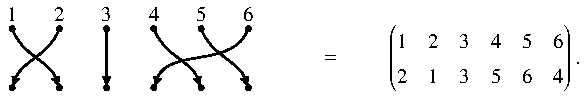
\includegraphics{chapters/50-permutationen/images/permutation.pdf}
\end{center}
Das neutrale Element hat die Matrix
\[
e = \begin{pmatrix}
1&2&3&4&5&6\\
1&2&3&4&5&6
\end{pmatrix}
\]
aus zwei identischen Zeilen.

Die Verknüpfung zweier solcher Permutationen kann leicht graphisch
dargestellt werden: dazu werden die beiden Permutationen
untereinander geschrieben und Spalten der zweiten Permutation
in der Reihenfolge der Zahlen in der zweiten Zeile der ersten
Permutation angeordnet.
Die zusammengesetzte Permutation kann dann in der zweiten Zeile
der zweiten Permutation abgelesen werden:
\begin{center}
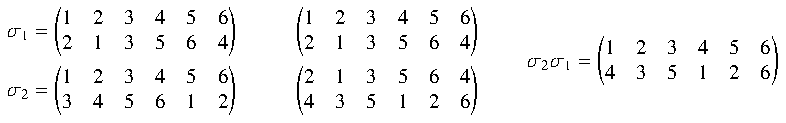
\includegraphics{chapters/50-permutationen/images/komposition.pdf}
\end{center}
Die Inverse einer Permutation kann erhalten werden, indem die beiden
Zeilen vertauscht werden und dann die Spalten wieder so angeordnet werden,
dass die Zahlen in der ersten Zeile ansteigend sind:
\[
\sigma = \begin{pmatrix}
1&2&3&4&5&6\\
2&1&3&5&6&4
\end{pmatrix}
\qquad\Rightarrow\qquad
\sigma^{-1}
=
\begin{pmatrix}
2&1&3&5&6&4\\
1&2&3&4&5&6
\end{pmatrix}
=
\begin{pmatrix}
1&2&3&4&5&6\\
2&1&3&6&4&5
\end{pmatrix}.
\]

\subsection{Zyklenzerlegung
\label{buch:subsection:zyklenzerlegung}}
Eine Permutation $\sigma\in S_n$ kann auch mit der sogenanten Zyklenzerlegung
\index{Zyklenzerlegung}%
analysiert werden.

\begin{definition}
Ein Zyklus $Z$ ist eine unter $\sigma$ invariante Teilmenge von $[n]$
minimaler Grösse.
\index{Zyklus}%
\index{invariante Teilmenge}%
\index{minimale Grösse}%
Die Zyklenzerlegung ist eine Zerlegung von $[n]$ in Zyklen
\[
[n]
=
\bigcup_{i=1}^k Z_i,
\]
wobei jede Menge $Z_i$ ein Zyklus ist.
\end{definition}

Zum Beispiel:
\begin{center}
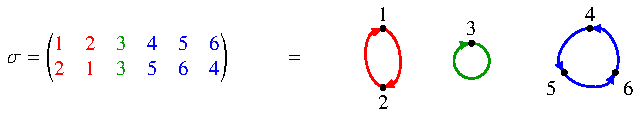
\includegraphics{chapters/50-permutationen/images/zyklenzerlegung.pdf}
\end{center}
Der folgende Satz stellt einen Algorithmus bereit, mit dem die
Zyklenzerlegung einer Permutation gefunden werden kann.

\begin{satz}
Sei $\sigma\in S_n$ eine Permutation. Der folgende Algorithmus findet
die Zyklenzerlegung von $\sigma$:
\begin{enumerate}
\item
$i=1$
\item
Wähle das erste noch nicht verwendete Element
\[
s_i=\min\biggl( [n] \setminus \bigcup_{j< i} Z_j\biggr)
\]
\item
Bestimme alle Elemente, die aus $s_i$ durch Anwendung von $\sigma$
entstehen:
\[
Z_i
=
\{ s_i, \sigma(s_i), \sigma(\sigma(s_i)), \dots \}
=
\{\sigma^k(s_i)\;|\; k\ge 0\}.
\]
\item
Falls $\bigcup_{j\le i} Z_j\ne [n]$, erhöhe $i$ um $1$ und fahre 
weiter bei 2.
\end{enumerate}
\end{satz}

Mit Hilfe der Zyklenzerlegung von $\sigma$ lassen sich auch
gewisse Eigenschaften von $\sigma$ ableiten.
Sei also $[n] = Z_1\cup\dots\cup Z_k$ die Zyklenzerlegung von $\sigma$.
Für jedes Element $x\in Z_i$ gilt $\sigma^{|Z_i|}(x) = x$.
Die kleinste Zahl $m$, für die $\sigma^m=e$ ist, das kleinste
gemeinsame Vielfache der Zyklenlängen:
\[
m = \operatorname{kgV} (|Z_1|,|Z_2|,\dots,|Z_k|).
\]
\index{kgV}
\index{kleinstes gemeinsames Vielfaches}

\subsection{Konjugierte Elemente in $S_n$}
Zwei Elemente $g_1,g_2\in G$ einer Gruppe heissen {\em konjugiert}, wenn
\index{konjugiert}
es ein Element $c\in G$ gibt derart, dass $cg_1c^{-1}=g_2$.
Bei Matrizen bedeutet dies, dass die beiden Matrizen durch
Basiswechsel auseinander hervorgehen.
Dasselbe lässt sich auch im Kontext der symmetrischen Gruppe sagen.

Seien $\sigma_1$ und $\sigma_2$ zwei konjugierte Permutationen in $S_n$.
Es gibt also eine Permutation $\gamma\in S_n$ derart, dass
$\sigma_1=\gamma\sigma_2\gamma^{-1}$ oder $\gamma^{-1}\sigma_1\gamma=\sigma_2$.
Dann gilt auch für die Potenzen
\begin{equation}
\sigma_1^k
=
(\gamma\sigma_2\gamma^{-1})^k
=
\gamma\sigma_2\underbrace{\gamma^{-1}
\gamma}_{\displaystyle=e}\sigma_2\underbrace{\gamma^{-1}
\gamma}_{\displaystyle=e}\sigma_2\underbrace{\gamma^{-1}\gamma}_{\displaystyle=e}
\cdots
\underbrace{\gamma^{-1}
\gamma}_{\displaystyle=e}\sigma_2\gamma^{-1}
=
\gamma\sigma_2^k\gamma^{-1}.
\label{buch:permutationen:eqn:konjpot}
\end{equation}
Ist $Z_i$ ein Zyklus von $\sigma_2$ und $x\in Z_i$, dann ist
$Z_i = \{ x,\sigma_2(x),\sigma_2^2(x),\dots\}$.
Die Menge $\gamma(Z_i)$ besteht dann aus dem Elementen
$\gamma(Z_i)=\{\gamma(x),\gamma(\sigma_2(x)),\gamma(\sigma_2^2(x)),\dots\}$.
Aus der Formel~\eqref{buch:permutationen:eqn:konjpot} folgt
$\sigma_1^k\gamma = \gamma\sigma_2^k$, also
\[
\gamma(Z_i)
=
\{\gamma(x),\sigma_1(\gamma(x)),\sigma_1^2(\gamma(x)),\dots\}.
\]
Somit ist $\gamma(Z_i)$ ein Zyklus von $\sigma_1$.
Die Permutation $\gamma$ bildet also Zyklen von $\sigma_2$ auf Zyklen
von $\sigma_1$ ab.
Es folgt daher der folgende Satz:

\begin{satz}
Seien $\sigma_1,\sigma_2\in S_n$ konjugiert $\sigma_1=\gamma\sigma_2\gamma^{-1}$
mit $\gamma\in S_n$.
Wenn $Z_1,\dots,Z_k$ die Zyklen von $\sigma_2$ sind, dann sind 
$\gamma(Z_1),\dots,\gamma(Z_k)$ die Zyklen von $\sigma_1$.
\end{satz}

Die Zyklenzerlegung kann mit der Jordan-Normalform
\index{Jordan-Normalform}%
(Abschnitt~\ref{buch:subsection:jordan-normalform})
einer Matrix verglichen werden.
Durch einen Basiswechsel, welcher durch eine ``Konjugation''
\index{Basiswechsel}%
von Matrizen ausgedrückt wir, kann die Matrix in eine besonders 
übersichtliche Form gebracht werden.
Wenn $\sigma$ die Zyklenzerlegung $Z_1,\dots,Z_k$ hat mit Zyklenlängen
$l_i=|Z_i|$, dann kann man die Menge $[n]$ wie folgt in Teilmengen
\begin{align*}
X_1 &= \{1,\dots, l_1\},
\\
X_2 &= \{l_1+1,\dots,l_1+l_2\},
\\
X_i &= \{l_1+\dots+l_{i-1}+1,\dots, l_1+\dots+l_i\}
\\
X_k &= \{l_1+\dots+l_{k-1}+1,\dots n\}
\end{align*}
zerlegen.
Sei $\sigma_2$ die Permutation, die in jeder der Mengen $X_i$ durch
zyklische Vertauschung der Elemente wirkt.
Indem man die Elemente von $Z_i$ in der Reihenfolge, in der sie durch
$\sigma_1$ erreicht werden, auf die Elemente $X_i$ abbildet, findet
man eine Permutation, die Zyklen von $\sigma_1$ in Zyklen von $\sigma_2$
überführt.

\begin{satz}
Wenn zwei Elemente $\sigma_1,\sigma_2\in S_n$ Zyklenzerlegungen mit den
gleichen Zyklenlängen haben, dann sind sie konjugiert.
\end{satz}

Ein Element $\sigma\in S_n$ ist also bis auf eine Permutation
vollständig durch die Länge der Zyklen von $\sigma$ charakterisiert.


